\chapter{Resultados de validação e seleção dos modelos promissores}
\label{cap:validacao}

\section{Resultados da hiperparametrização}
\label{sec:busca}

As 25 tentativas levaram 6,2 minutos (23 completas, 2 podadas). A Figura~\ref{fig:optuna} mostra a evolução da busca e a importância dos hiperparâmetros; a Tabela~\ref{tab:top5}, as cinco melhores tentativas. O espaço é pouco sensível perto do ótimo (as 17 melhores ficam entre 0,597 e 0,600), e o que mais prejudica é a regularização forte: as piores tentativas combinam L2 alto ($> 10^{-3}$) com taxa de aprendizado baixa, e L1 e L2 aparecem como os mais importantes na fANOVA por causa dessas falhas, não de sensibilidade perto do ótimo. O lote de 512 dominou a partir da tentativa 6 e o sobreajuste é pequeno em todas (\textit{gap} de Macro F1 abaixo de 0,016).

\begin{figure}[!htbp]
  \centering
  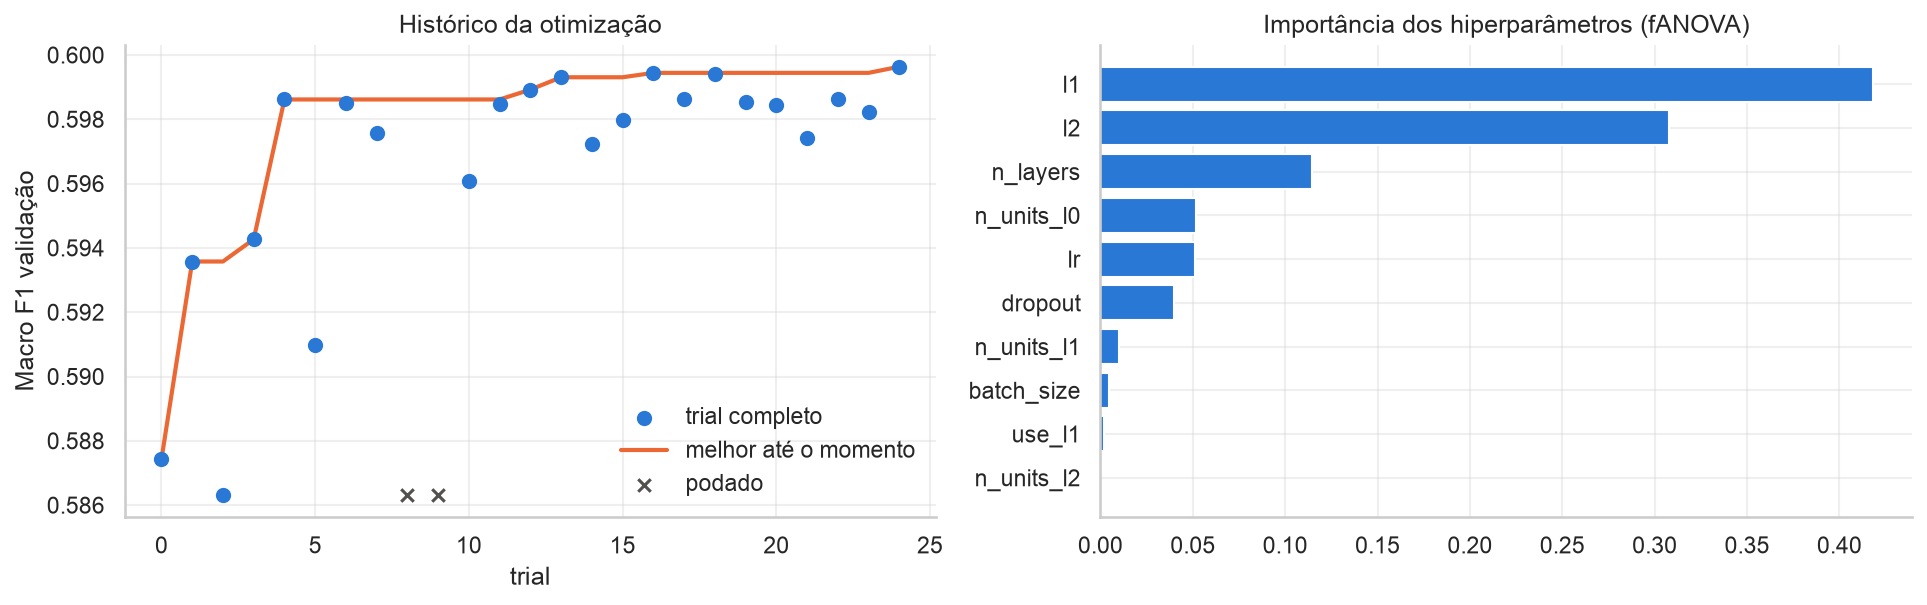
\includegraphics[width=0.7\textwidth]{figuras/10_optuna}
  \caption{Histórico da busca e importância dos hiperparâmetros (fANOVA)}
  \label{fig:optuna}
  \fontefig{Elaborado pelo autor}
\end{figure}

\begin{table}[!htbp]
\caption{Cinco melhores tentativas do Optuna (Macro F1 na validação)}
\label{tab:top5}
\begin{center}
\scriptsize
\setlength{\tabcolsep}{4pt}
\begin{tabular}{ccccccccc}
\hline
\textbf{Tentativa} & \makecell{\textbf{Macro F1}\\\textbf{val}} & \makecell{\textbf{Camadas}\\\textbf{ocultas}} & \textbf{Dropout} & \makecell{\textbf{Taxa de}\\\textbf{aprendizado}} & \textbf{L2} & \textbf{L1} & \textbf{Parâmetros} & \textbf{Gap F1} \\ \hline
24 & \textbf{0,5996} & 172 & 0,24 & $4{,}6 \cdot 10^{-4}$ & $1{,}1 \cdot 10^{-5}$ & --- & 34.059 & 0,008 \\
16 & 0,5994 & 215 $\rightarrow$ 25 & 0,32 & $7{,}2 \cdot 10^{-4}$ & $1{,}2 \cdot 10^{-5}$ & $1{,}3 \cdot 10^{-7}$ & 47.403 & 0,016 \\
18 & 0,5994 & 219 $\rightarrow$ 17 & 0,40 & $9{,}3 \cdot 10^{-4}$ & $8{,}0 \cdot 10^{-6}$ & $1{,}1 \cdot 10^{-7}$ & 46.499 & 0,008 \\
13 & 0,5993 & 228 $\rightarrow$ 19 & 0,17 & $4{,}8 \cdot 10^{-4}$ & $6{,}0 \cdot 10^{-5}$ & --- & 48.871 & 0,014 \\
12 & 0,5989 & 253 $\rightarrow$ 19 & 0,14 & $3{,}0 \cdot 10^{-4}$ & $5{,}0 \cdot 10^{-5}$ & --- & 54.221 & 0,012 \\ \hline
\end{tabular}
\end{center}
\fontetab{Elaborado pelo autor. Lote de 512 em todas. Gap F1 = Macro F1 de treino menos o de validação, na melhor época}
\end{table}

\section{Efeito da largura e da profundidade}
\label{sec:largura}

Para isolar o efeito da arquitetura, 9 redes foram treinadas na subamostra de 300 mil linhas variando só a profundidade (1, 2 ou 3 camadas) e a largura (32, 128 ou 256 neurônios), com os demais hiperparâmetros fixos (Figura~\ref{fig:largura-controlado}). A amplitude total é pequena (0,0044 de Macro F1) e, dentro dela, a largura pesa mais que a profundidade: com 32 neurônios as redes ficam entre 0,595 e 0,597 (subajuste leve), de 32 para 128 o ganho é de até 0,004, e de 128 para 256, de cerca de 0,001. Mais camadas não ajudam: com 128 ou 256 neurônios, 1 camada é igual ou melhor que 2 e 3, que atingem o melhor resultado na época 4 ou 5 e depois só aumentam o \textit{gap}. A rede 3 $\times$ 256 tem 182 mil parâmetros e não supera a 1 $\times$ 256, com 51 mil.

\begin{figure}[!htbp]
  \centering
  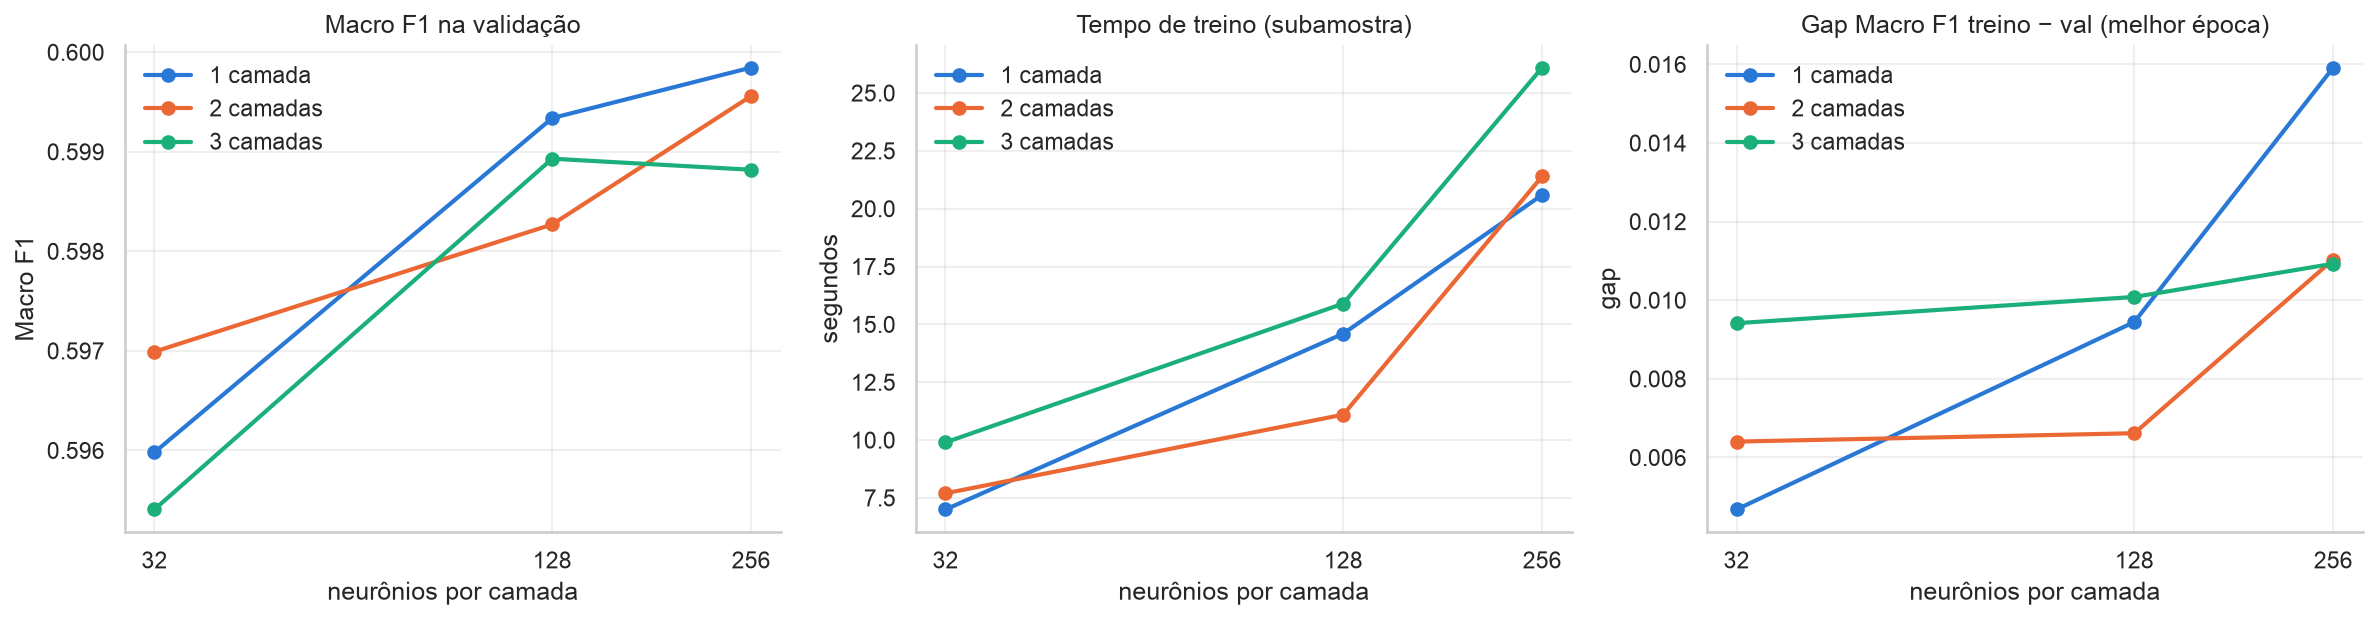
\includegraphics[width=0.85\textwidth]{figuras/10b_largura_profundidade_controlado}
  \caption{Experimento controlado de largura $\times$ profundidade (Macro F1 de validação, tempo e \textit{gap})}
  \label{fig:largura-controlado}
  \fontefig{Elaborado pelo autor}
\end{figure}

\section{Efeito da regularização}
\label{sec:regularizacao}

A arquitetura de M2 foi treinada na subamostra de 300 mil linhas por 25 épocas sem parada antecipada, com cada técnica isolada e com três referências (Tabela~\ref{tab:regularizacao} e Figura~\ref{fig:ablacao-reg}). Sem regularização a rede memoriza o treino (\textit{gap} de 0,060 e validação caindo após a 5\textsuperscript{a} época). O dropout é o que mais ajuda, e a combinação do Optuna é essencialmente esse dropout. L2 e L1 moderados reduzem o \textit{gap} sem melhorar a validação. O BatchNorm sozinho acelera o treino e antecipa o sobreajuste (melhor época 3, \textit{gap} de 0,094); não é regularização por si \cite{geron2019} e ficou fora dos finais. A regularização forte elimina o \textit{gap} à custa do desempenho: subajuste. Simulando a parada antecipada sobre essas curvas, a paciência 1 para cedo demais e perde até 0,008; com paciência 4 ou 5 as três configurações recuperam o melhor valor das 25 épocas, o que justifica os valores usados.

\begin{table}[!htbp]
\caption{Regularização técnica por técnica (25 épocas, sem parada antecipada)}
\label{tab:regularizacao}
\begin{center}
\scriptsize
\setlength{\tabcolsep}{3pt}
\begin{tabular}{P{3.3cm} c c c c P{4.6cm}}
\hline
\textbf{Configuração} & \makecell{\textbf{Macro F1}\\\textbf{treino}\\\textbf{(última)}} & \makecell{\textbf{Macro F1}\\\textbf{val}\\\textbf{(última)}} & \makecell{\textbf{Melhor}\\\textbf{Macro F1}\\\textbf{val (época)}} & \makecell{\textbf{Gap}\\\textbf{(última)}} & \textbf{Diagnóstico} \\ \hline
Sem regularização & 0,644 & 0,584 & 0,598 (5) & \textbf{0,060} & sobreajuste: o treino sobe sem parar e a validação cai depois da 5\textsuperscript{a} época \\ \hline
Só dropout (0,32) & 0,630 & 0,595 & 0,599 (12) & 0,034 & técnica isolada mais eficaz \\ \hline
Só L2 ($10^{-4}$) & 0,627 & 0,589 & 0,598 (6) & 0,039 & reduz o \textit{gap}, mas a validação ainda cai \\ \hline
Só L1 ($10^{-5}$) & 0,622 & 0,591 & 0,598 (8) & 0,031 & efeito parecido com o do L2 \\ \hline
Só BatchNorm & 0,667 & 0,573 & 0,596 (3) & \textbf{0,094} & antecipa o sobreajuste \\ \hline
Combinação do Optuna (dropout 0,32, L2 $1{,}2 \cdot 10^{-5}$, L1 $1{,}3 \cdot 10^{-7}$) & 0,626 & 0,597 & \textbf{0,600} (16) & 0,030 & equilíbrio: menor \textit{gap} sem subajuste e melhor validação \\ \hline
Regularização forte (dropout 0,5, L2 $10^{-2}$) & 0,565 & 0,564 & 0,578 (15) & 0,001 & subajuste: treino e validação colados e baixos \\ \hline
\end{tabular}
\end{center}
\fontetab{Elaborado pelo autor}
\end{table}

\begin{figure}[!htbp]
  \centering
  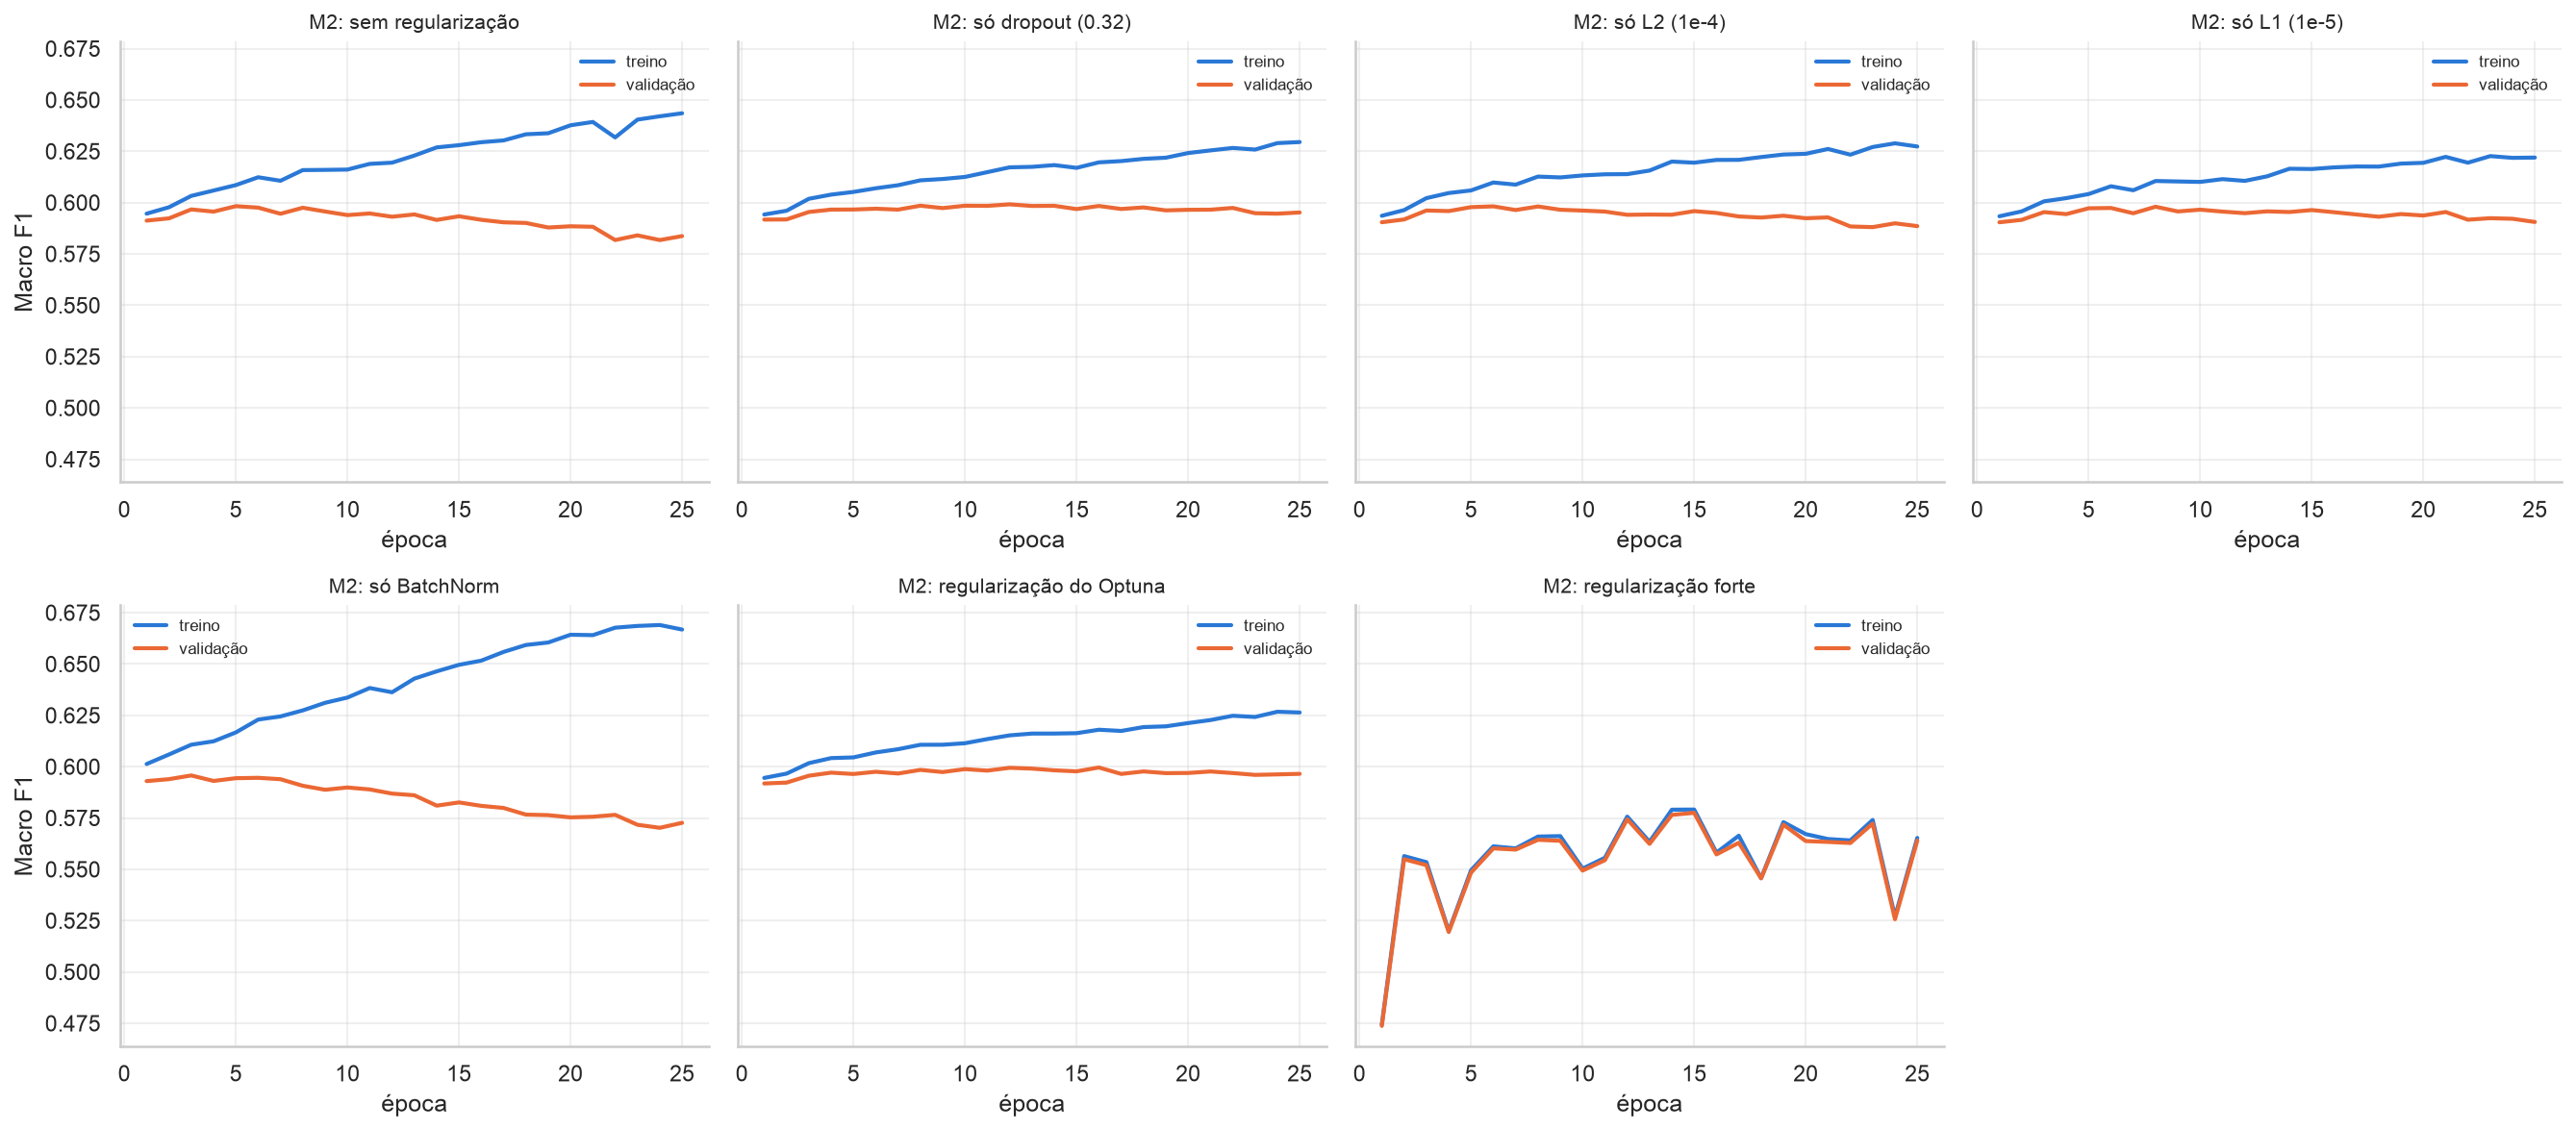
\includegraphics[width=0.7\textwidth]{figuras/13_ablacao_regularizacao}
  \caption{Macro F1 de treino e validação por época, por técnica de regularização}
  \label{fig:ablacao-reg}
  \fontefig{Elaborado pelo autor}
\end{figure}

\section{Seleção dos modelos finalistas}
\label{sec:finalistas}

As três melhores tentativas com arquiteturas distintas (24, 16 e 18 na Tabela~\ref{tab:top5}) definem os finalistas M1, M2 e M3 (Quadro~\ref{qua:finais}). A busca convergiu para redes rasas e largas: uma camada de 172 neurônios ou duas camadas em formato pirâmide (cerca de 215 e 20 neurônios), sempre com dropout entre 0,24 e 0,40, L2 em torno de $10^{-5}$, L1 desligado ou quase nulo e lote 512. Três variações são comparadas para verificar se a segunda camada traz algum ganho no treino com a base completa.

\begin{quadro}[!htbp]
\caption{Arquiteturas finalistas resultantes da hiperparametrização}
\label{qua:finais}
\begin{center}
\scriptsize
\setlength{\tabcolsep}{4pt}
\begin{tabular}{|c|c|c|c|c|c|c|c|}
\hline
\textbf{Modelo} & \textbf{Tentativa} & \textbf{Arquitetura} & \textbf{Parâmetros} & \textbf{Dropout} & \makecell{\textbf{Taxa de}\\\textbf{aprendizado}} & \textbf{L2} & \textbf{L1} \\ \hline
M1 & 24 & 194 $\rightarrow$ 172 $\rightarrow$ 3 & 34.059 & 0,24 & $4{,}6 \cdot 10^{-4}$ & $1{,}1 \cdot 10^{-5}$ & --- \\ \hline
M2 & 16 & 194 $\rightarrow$ 215 $\rightarrow$ 25 $\rightarrow$ 3 & 47.403 & 0,32 & $7{,}2 \cdot 10^{-4}$ & $1{,}2 \cdot 10^{-5}$ & $1{,}3 \cdot 10^{-7}$ \\ \hline
M3 & 18 & 194 $\rightarrow$ 219 $\rightarrow$ 17 $\rightarrow$ 3 & 46.499 & 0,40 & $9{,}3 \cdot 10^{-4}$ & $8{,}0 \cdot 10^{-6}$ & $1{,}1 \cdot 10^{-7}$ \\ \hline
\end{tabular}
\end{center}
\fontequa{Elaborado pelo autor. Arquitetura: entrada $\rightarrow$ camadas ocultas $\rightarrow$ saída; ReLU nas ocultas, softmax na saída, Adam e lote 512 em todos}
\end{quadro}
